% 来源：1991三南原卷，PDF第1页（印刷页41），第14题。
% 数学化重建：按原图周期、幅值、x=1处下降过零及给定选项使用sin(1-x)。
% 保留原图的坐标标号和虚线；不增加未给出的刻度或题设条件。
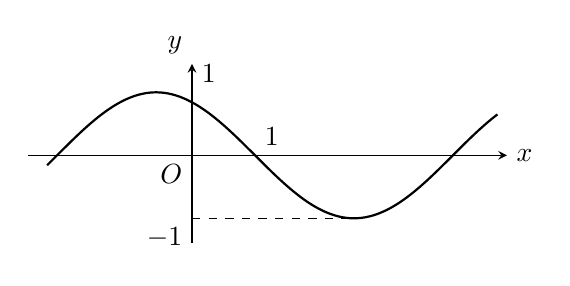
\begin{tikzpicture}[x=0.8cm,y=0.8cm,>=stealth]
  \draw[->] (-2.6,0)--(5,0) node[right] {$x$};
  \draw[->] (0,-1.4)--(0,1.45) node[above left] {$y$};
  \node[below left] at (0,0) {$O$};
  \node[above right] at (0,1) {$1$};
  \node[below left] at (0,-1) {$-1$};
  \node[above right] at (1,0) {$1$};
  \draw[dashed] (0,-1)--({1+pi/2},-1);
  \draw[thick,domain=-2.3:4.85,samples=120,smooth]
    plot (\x,{sin((1-\x) r)});
\end{tikzpicture}
